
In this chapter, we discuss results on the mapping of temporal data obtained from a discrete-dynamical system onto a different space through the notion of a driven dynamical system. 
We also consider the conditions a driven system should possess to avoid adding distortion to its state-space representation. We then describe the \emph{single-delay dynamics} (SDD) of the system and finally recall conditions on the driven system so that the SDD are conjugate (or at least semi-conjugate) to the underlying system. 
The SDD can then be used to forecast and reconstruct the underlying system. 

\section{Nonautonomous and Driven Dynamical Systems}

\begin{Definition}
  [\bf Nonautonomous Dynamical System (adopted from~\cite{Manju_ESP})]\label{Dfn_NDS}\rm
  A nonautonomous dynamical system (NDS) on a space $X$ is simply a dynamical system comprising a family of maps ${\{g_n\}}_{n \in \mathbb{Z}}$ where $g_n(\ldotp):=g(u_n,\ldotp):X\to{X}$ is continuous. Each $g_n$ arises as a consequence of an input $u_n$ from the input space $U$, a topological space. 
\end{Definition}

We immediately recall the figure first defined in\eqref{eqn_conjugacy}  and remind ourselves of our ultimate goal to learn a system that is conjugate to an underlying or unknown dynamical system $(U,T)$ by making use of the measurements obtained from  the unknown system. 
See this sketched in the diagram~\ref{UV_conjugacy}

%#####################################
\begin{equation}
  % \begin{center}
    \centering
    \psset{arrows=->, arrowinset=0.25, linewidth=0.6pt, nodesep=3pt, labelsep=2pt, rowsep=0.7cm, colsep = 1.1cm, shortput =tablr}
    \everypsbox{\scriptstyle}
    \begin{psmatrix}\label{UV_conjugacy}
    U & U\\%
    V & V.
    %%%
    %  \ncline{1,1}{1,2}^{T} 
    %  \ncline{1,1}{2,1} <{\phi}
    %   \ncline{2,1}{2,2}^{S}
    %  \ncline{1,2}{2,2} > {\phi}
    \end{psmatrix}
    %#####################################
    % \end{center}
\end{equation}


To find a function $\phi$, the need now arises to consider a so-called driven dynamical system, a special case of a nonautonomous dynamical system. Two spaces are considered: input is taken from an input space $U$ and the state of a space $X$ is updated. (Previously, only the state was considered.)
We do this to mimic the true conditions. By accounting for an extrogenous input sequence in $U$ which can also influence the  system-state at a specific time-step, it produces more general models than an autonomous system.

\begin{Definition}
  [\bf Driven, Compactly Driven Dynamical System]\label{Dfn_DDS} \rm
A driven dynamical system comprises two topological metric spaces $U$, $X$ and a continuous function  $g:U\times{X}\to{X}$ where $g(u_n, x_n)=x_{n+1}$.
If the input space $U$ is compact, we refer to the system as compactly driven. 
\end{Definition}

The update equation $x_{n+1} = g(u_n,x_n)$ for $n \in\mathbb{Z}$, input $u_n$ from $U$ and state $x_n$ belonging to $X$ (a compact space) generate the dynamics on X. 
Abbreviated, we refer only to the \textit{driven system $g$}, where all other entities are understood implicitly.

Notably, a nonautonomous dynamical system can be generated from $U$; any input $\overline{u}$, a bi-infinite sequence from $U$, gives rise to the sequence of self-maps ${\{g(u_n, \cdot)\}}_{n\in\mathbb{Z}}$ contained in $X$.
Physically, one may think of this bi-infinite sequence as referring to a system that has been running for an extended period at the time of the first measurement taken from the system (alternatively, the first time a probe is inserted into the system to take an observation)

\begin{Definition}
  [\bf Entire Solution]\label{Dfn_Soln} \rm
  A sequence ${\{x_n\}}_{n\in\mathbb{Z}}\subset X$ is called an entire solution (or simply a solution) of the driven system  $g$ with input $\overline{u}$ when it satisfies 
  \begin{equation}
    g(u_{n-1}, x_{n-1})=x_n \text{ for all }n\in\mathbb{Z}
  \end{equation}
  
\end{Definition}

It is important to emphasise that a sequence $\{x_n\}$ satisfying the update equation above can only be a solution if $x_n\in{U}$ holds for all $n\in\mathbb{Z}$ and just for $n>0$. Consider the example below.

\begin{Example}\label{ex_halfux} \rm
  The only solution  ${\{x_n\}}_{n\in\mathbb{Z}}$ to the driven system  $g(u,x)=\frac{ux}{2}$, where $X=[0,1]$, $U=[0,1]$,  is the zero solution $x_n\equiv0$.
  To see this, consider any $x_n=a\in[0,1]$ where $a\neq{0}$.  Let $\overline{u}\in{U}$ be an non-zero constant sequence, say $u_n=0.5$. 
  The driven system may be rewritten as $x_{n-1}=\frac{2x_n}{u_{n-1}}=4x_n$ and the  iterates of $x_n$ in backward time will increase by a factor of 4 at each timestep. 
  Thus for some $m\leq{n}$,  $1<x_m$ i.e. $x_m\notin{X}$. So ${\{x_n\}}_{n\in\mathbb{Z}}$ is not a solution and it follows that the only possible solution is the zero solution.
\end{Example}
% \ednote{Nicely written! Thank you}


A system may also have multiple solutions, as evidenced in the example below.

\begin{Example}\label{Ex_exp} \rm 
  Consider the driven system $g(u,x)=x^2$ for $X=[0,1]$, $U=\mathbb{R}$. The system has an uncountable number of solutions, as there exists a solution for every $x\in{X}$ which also passes through the point $x$ and $\lim_{n\to\infty}x_n=0$, $\lim_{n\to{-}\infty}x_n=1$.  
 The proof is deferred to immediately after the next paragraph (see~\ref{rem_proofEx}).
\end{Example}

As the solutions to a driven system are considered an important entity, we next identify a subspace $X_U$ of $X$ that contains all possible solutions. To realize such a subspace of a driven system $g$, the concept of a reachable set is defined.

\begin{Definition}
  [\bf Reachable Set]\label{Dfn_ReachableSet}\rm
The reachable set of a driven system $g$ is exactly the union of all the elements of all the (entire) solutions, i.e., 
\begin{equation}
  X_U :=\Big \{x \in X:  x = x_k \mbox{ where  $\{x_n\}$  is a solution for some  $\bar{u}$} \Big \}.  
\end{equation}

The set of all reachable states at a specific time $n$ for input $\overline{u}$ is denoted by $X_n(\overline{u})$
\end{Definition}

The reachable set itself can defined independently from $g$ possessing the ESP/USP. Note that $x\in{X_n(\overline{u})}$ if and only $g$ has a solution $\{x_k\}$ for $x_n=x$ and input $\overline{u}$, a result proved in nonautonomous dynamical systems literature~\cite{manjunath2014dynamics, manjunath2013echo}. \ednote{B: Adjusted sentence and cited}

The set $X_n(\overline{u})$ is precisely the set of points $x$ through which some entire solution $\Psi$ passes at time $n$. We can give an alternate formulation of the set $X_n(\overline{u})$. 
Now suppose, we for some fixed input 
$\overline{u}$, we define $g_i = g(u_i,\cdot)$ for all $i\in \mathbb{Z}$, then the set of states
\begin{equation} \label{eqn_association}
X_{n,i}(\overline{u}) := g_{n-1} \circ \cdots g_{i+1} \circ g_i(X).
\end{equation}

The set $X_{n,i}(\overline{u})$ being the image of a finite composition of
continuous maps is compact whenever $X$ is compact. Also $X_{n,i}(\overline{u})$ is
nonempty.  Further, $X_{n,i}(\overline{u}) \supset X_{n,i-1}$. Hence $\bigcap_{i<n}
X_{n,i}(\overline{u})$ is a nested intersection of closed nonempty subsets, and
whenever $X$ is compact, the intersection is nonempty. We say $g$ is a topological contraction if $\bigcap_{i<n}X_{n,i}(\overline{u})$ is a singleton subset of $X$ for each $\overline{u}$. 

It turns out that $\bigcap_{i<n}X_{n,i}(\overline{u})$ is identically equal to $X_n((\overline{u})$ that we had defined earlier. This will lead to a result (see~\cite{manjunath2013echo}) that \textit{$g$ being a topological contraction is equivalent to the existence of a exactly one entire solution.}

% \begin{Definition}
%   [\bf Topological Contraction]\label{Dfn_TopContr}\rm
%   A function $g:U\times{X}\to{X}$ is a topological contraction if for all $n\in\mathbb{Z}$ and all $\overline{u}\subset{U}$, $X_n(\overline{u})$ is a singleton subset of $X$.  
% \end{Definition}

\begin{Remark}
  [\bf Proof of Example~\ref{Ex_exp}]\label{rem_proofEx} \rm
  For the driven system,  
  $g(u,x)=x^2$ the evolution does not depend on the input at all. Hence $g(u,x)$ can be written as a single map $f(x)=x^2$ which is a homeomorphism on $[0,1]$. A left-infinite orbit is defined and it converges to $1$ while the right-infinite orbit converges to $0$. Or in other words the iterates of $f^{-1}$ converges to $1$ while the iterates of $f$ converge to $0$ 
\end{Remark}

Thus far, it has been demonstrated that a system may have one or more solutions; one may ask if a driven system always has a solution and, if so, whether it satisfies specific properties such as uniqueness. 
Should the driven system be compact, existence follows immediately, as shown in the following result.

\begin{Theorem}\label{Thm_CompactExistence}
 Let $g$ be a driven system.  If $X$ is compact then for each input $\overline{u}$, there exists at least one solution to the driven system $g(\ldotp, x)$
\end{Theorem}
{\bf Proof.} May be found in~\cite{kloeden2011nonautonomous, manjunath2014dynamics, manjunath2013echo}
% One may easily construct many systems with trivial solution-sets, such as $g(u,x)=x$ which has only the constant solution $x$ and so for $U=[-1,1]$, the system would have no solution if $|x|>1$. To refine the scenario, we consider only systems with unique solutions. 
\section{Unique Solution Property}

\begin{Definition}
  [\bf Unique Solution Property]\label{Dfn_usp}\rm
  A driven system $g$ is said to have the Unique Solution Property (USP) if for each input $\overline{u}$ there exists exactly one solution. 
  Alternatively we may formulate the USP as follows: $g$ has the Unique Solution Property if there exists a well-defined map $\Psi:{U}\to{X}$, with $\Psi({\overline{u}})$ denoting the unique solution.
\end{Definition}

One of the first results obtained after defining the USP is that every solution will attract different initial conditions towards the component parts of the solution.
If $g$ has the USP, then any solution to $g$ is also a uniform attractor in nonautonomous dynamical systems literature~\cite{Manju_Nonlinearity}. The discussion on nonautonomous attractors is beyond the scope of this project, and we refer the reader to~\cite{Manju_ESP, esann2012ids} for further reading. 

% Paraphrased.
%Additionally, $g$ having the USP is in our context also equivalent to $g$ being a topological contraction \cite{manjunath2021universal}, or alternatively also that $g$ exhibits the Echo State Property (ESP). 

In the majority of Reservoir Computing (RC) literature- a machine learning approach- where the input is mapped onto a different but higher dimensional through a system called the reservoir and a readout that measures the state of the reservoir is trained, a notion of forgetting the states of the reservoir asymptotically is often used.  

% \ednote{How should I explain/qualify RC better here? It's mentioned without really explaining. M: Have put it in one sentence; just to let you know people use optical devices to map signal into a ``reservoir". B: Thanks!}, 
Concepts like the ESP,  fading memory~\cite{boyd1985fading} are some of these notions.  
If $g$ possesses the ESP (equivalent in our context to the USP), the we are guaranteed that the whole of an input's left-infinite history will exactly determine the current system state; i.e. there is only ever the possibility of a single reachable state at a given instance of time~\cite{jaeger2001echo,Manju_2020}.
% Defined formally, the ESP is intrinsically linked to an input (see \cite{Manju_ESP}) Unfortunately, definitions and results concerning the ESP do not have much practical benefit since a relationship between the network's response and the temporo-statistical properties of the input are not directly described. A more detailed presentation may be found in~\cite{jaeger2001echo}.

% We do however consider it important to mention that the ESP is also often discussed in terms of a stability property that holds for all inputs of a system~\cite{manjunath2020stability} and, furthermore, plays a key role in the design and training of recurrent neural networks(RNN) within the field of RC \cite{Manju_ESP}.
Beyond forgetting the past states the ESP is also often discussed in terms of a stability property that is nearby inputs create close by responses (solutions), a concept called input-related stability~\cite{manjunath2020stability} and, furthermore, plays a key role in the robustness of recurrent neural networks (RNN), a component of the implementation discussed in~\ref{ch5}.

\section{Conjugacies}

Having already defined the reachable set $X_U$ as the collection of all elements of all entire solutions, we pause briefly in order to fix additional notation.
Defining $\cev{u}^{n}:=(\ldots,u_{n-2} ,u_{n-1})$ as the left-infinite subsequence of an input up until time $n$, $\overleftarrow{U}$ is then the notation for all these left-infinite sequences in $U$. 
Moreover, $\cev{u}^{n}v:=(\ldots,u_{n-2} ,u_{n-1}, v)$ will symbolise the input up to time $n$ with $v \in U$ being the specific input value at time $n$. 
The introduction of a new input at time $n$ can be described by the mapping $\sigma_v:   \cev{u}^{n} \mapsto \cev{u}^{n}v$. 
The right-shift map, $r\overleftarrow{U}\to\overleftarrow{U}$, of an input sequence is defined $r: (\cdots, u_{-2},u_{-1}) \mapsto(\cdots, u_{-3},u_{-2})$

The question now assumes the form: Can we establish a semi-conjugacy for the driven system $g$ as presented below.

\begin{equation}  \label{Scomm_h}
  %    \[ 
      \psset{arrows=->, arrowinset=0.25, linewidth=0.6pt, nodesep=3pt, labelsep=2pt, rowsep=0.7cm, colsep = 1.1cm, shortput =tablr}
   \everypsbox{\scriptstyle}
   \begin{psmatrix}
   \overleftarrow{U} & \overleftarrow{U}\\%
   X_U & X_U.
   %%%
  %  \ncline{1,1}{1,2}^{\sigma_v} \ncline{1,1}{2,1} <{h}
  %  \ncline{1,2}{2,2} > {h}
  %  \ncline{2,1}{2,2}^{g(v,\cdot)}
   \end{psmatrix}
  % \]
  \end{equation} 	


We proceed to consider a specific subclass of conjugacies.

  \begin{Definition}
    [\bf Universal Semi-Conjugacy]\label{Def_UnivSemiConj} \rm
    Given a driven system $g$, we  call a continuous and surjective map $h : \overleftarrow{U} \to X_U$ a universal semi-conjugacy if  diagram~\ref{Scomm_h} commutes for all $v \in U$.
  \end{Definition}

  If the universal semi-conjugacy $h$ exists (i.e. the diagram in~\ref{Scomm_h} commutes) then the solution $\Psi(\bar{u})$ will intuitively have no more ``complexity' than the input $\bar{u}$.

But does such a function $h$ for the above driven system $g$ above exist? Whenever $g$ has the USP and $\Psi(u)={\{x_n\}}_{n\in\mathbb{Z}}$ it follows that $h$, defined by  $h(\cev{u}_n):=g(u_n,x_{n-1})=x_n$, will satisfy the semi-conjugacy in the graph above~\ref{Scomm_h}.
Regrettably, such a continuous mapping $h$ is not guaranteed to exist when $g$ does not have the USP~\cite[Lemma 5]{Manju_Nonlinearity}.
Note that even when $h$ does exist, we are not guaranteed its injectivity. Considering again example~\ref{ex_halfux}, we see that even if $h$ were to exist, it could not be injective as $X_U=\{0\}$.

Re-sketching the commutativity diagram~\ref{Scomm_h} above by replacing $X_U$ by its left-infinite sequence space $\overleftarrow{X}_U$, we obtain the diagram below. In this case, the function $H:\overleftarrow{U}\to\overleftarrow{X}_U$, a map that is both continuous and surjective, is called a \emph{causal mapping} that is defined next. 

\begin{Definition}
  [\bf Causal Mapping]\label{Def_CausMap}
  A continuous, surjective map $H:\overleftarrow{U}\to\overleftarrow{X}_U$ such that \[H\circ\tilde{g}_v=\sigma\circ{H}\] holds for all $v \in U$ where $\tilde{g}_v$ maps $(\ldots, u_{-2}, u_{-1})$ to $(\ldots, u_{-2}, u_{-1}, g(v, u_{-1}))$ is called a causal mapping.
\end{Definition}

\begin{equation} \label{SCausal_H}
    %    \[ 
        \psset{arrows=->, arrowinset=0.25, linewidth=0.6pt, nodesep=3pt, labelsep=2pt, rowsep=0.7cm, colsep = 1.1cm, shortput =tablr}
     \everypsbox{\scriptstyle}
     \begin{psmatrix}
     \overleftarrow{U} & \overleftarrow{U}\\%
     \overleftarrow{X}_U & \overleftarrow{X}_U.
     %%%
    %  \ncline{1,1}{1,2}^{\sigma_v} \ncline{1,1}{2,1} <{h}
    %  \ncline{1,2}{2,2} > {h}
    %  \ncline{2,1}{2,2}^{\tilde{g}_v}
     \end{psmatrix}
    % \]
  \end{equation} 	

 \begin{Theorem}
  For a compactly driven system, a causal mapping $H$ exists if and only if $g$ has the USP. 
\end{Theorem}
{\bf Proof.}  See~\cite[Th.3]{manjunath2013echo}.

The driven system $g$ can induce an embedding of $\overleftarrow{U}$ in $\overleftarrow{X}$ as follows: 
If the causal mapping $H:\overleftarrow{U}{\to}{\overleftarrow{X}_U}$ is injective (in addition to being surjective), it becomes the embedding of $\overleftarrow{U}$ in $\overleftarrow{X}$ induced by the driven system $g$. 
The continuity of $H^{-1}$ follows from the fact that $H$ is itself a continuous and surjective mapping of a compact space $\overleftarrow{U}$ in a Hausdorff space.
and we refer to the map $H$ as a \emph{causal embedding}. 
\ednote{B: edited the sentence here}

When $g$ has the USP, the diagram below (adopted from~\cite{Manju_Nonlinearity}) illustrates the operation of the mappings $h$ and $H$. The mapping $h:\overleftarrow{U}\to{X_U}$ is also considered an observable as mentioned in the introduction of Chapter~\ref{ch3}).  

\begin{figure}[ht]
  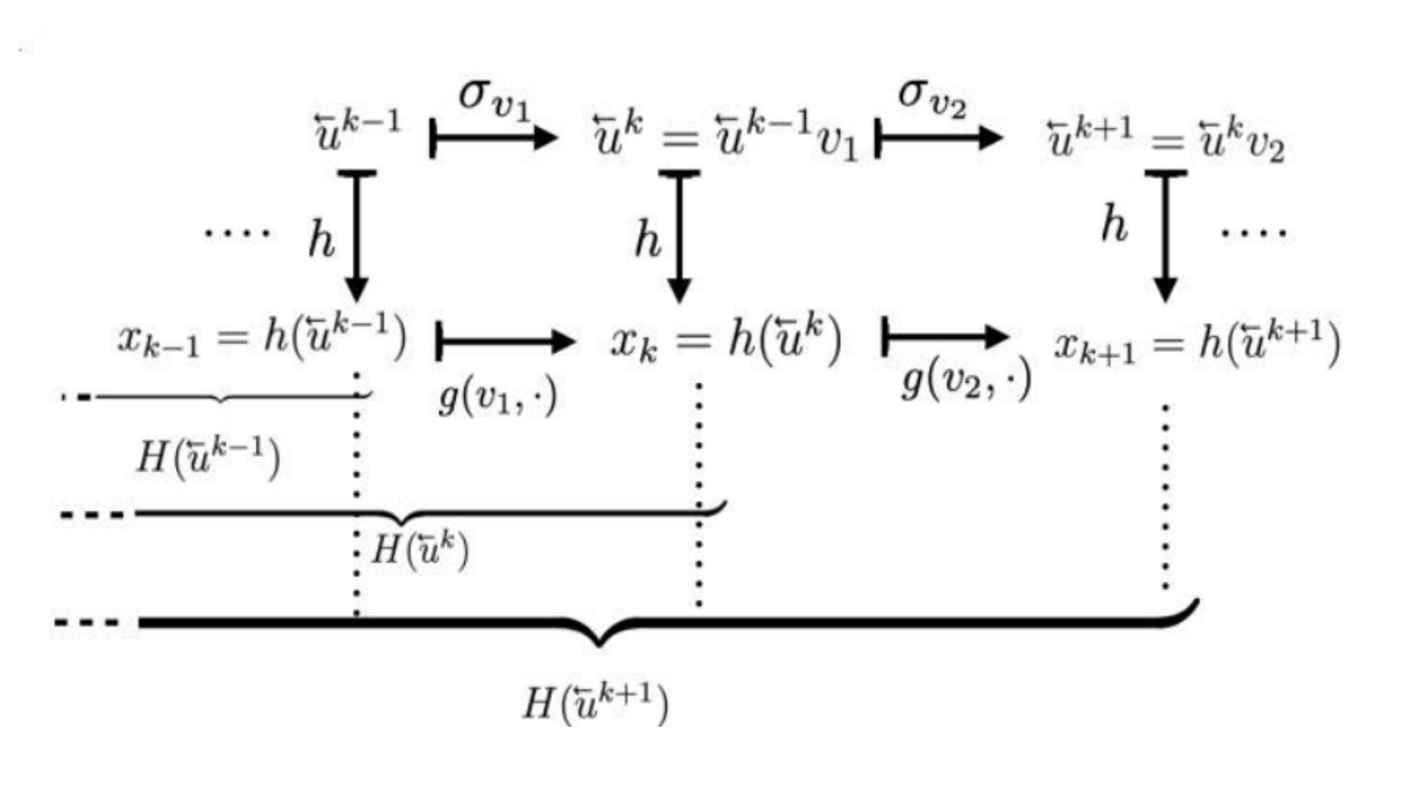
\includegraphics[scale=0.4]{Graphs/_actionofh_H.eps}
  \centering
  \captionof{figure}{Ladder-like behaviour of $h$ and $H$ to illustrate the causal mapping. (Figure reproduced from~\cite{Manju_Nonlinearity}) }
 \label{fig:actionh_H}
\end{figure}

The function $H$ contains a countably infinite number of coordinate (or factor maps) since its codomain is $\overleftarrow{X}_U$.  
As it is not practically feasible to consider a left-infinite sequence in $X_U$ (in other words an element of  $\overleftarrow{X}_U$) for learning, we wish to restrict the inputs we consider to a subspace of $\overleftarrow{U}$. 
Particularly, we restrict our attention to the  so-called inverse-limit space of a dynamical system and hope to embed it within some finite product of $X$. 

%We wish to explore the possibility of establishing a conjugacy rather than a mere semi-conjugacy and therefore are interested in the restriction of inputs to the left-infinite orbits of a dynamical system.

The left-infinite orbit space is significant because a great amount of information about the original system can be gleaned from its topological structure~\cite{ingram2011inverse,Manju_IEEE}. 
The formal topological structure for the inverse-limit space of a chaotic dynamical system is complicated, and further discussion is relegated to~\cite{kennedy2008inverse_limit, ingram2011inverse}.
Broadly, we may conceive of the inverse-limit system of a dynamical system as a subspace of an infinite-dimensional space where each point in the inverse-limit space corresponds to a backward orbit of the map $T$. 
Following~\cite{manjunath2021universal, ingram2011inverse} we provide a definition:

\begin{Definition}
  [\bf Inverse-Limit Space, Inverse-Limit System]\label{Dfn_InverseL}\rm
 The subset $\widehat{U}_T\subset \overleftarrow{U}$ defined by 
 \begin{equation}
  \widehat{U}_T: = \{ (\ldots,u_{-2},u_{-1}): Tu_{i} = u_{i+1}\}  
 \end{equation}
 is called the inverse-limit space of $(U,T)$.
 The self-map $\widehat{T}$  induced by $T$ on $\widehat{U}_T$  is defined by 
 \begin{equation}
  \widehat{T}: (\ldots,u_{-2},u_{-1}) \mapsto  (\ldots,u_{-2},u_{-1},T(u_{-1}))  
 \end{equation}
 and the resulting dynamical system $(\widehat{U_T}, \widehat{T})$ is called the inverse-limit system of $(U,T)$.
\end{Definition}

The inverse-limit space is well-defined since $T : U \to{U}$ is surjective by assumption.
We now get to the concept of embedding the inverse limit-space of the dynamical system in $X \times X$. 
\begin{Definition} \rm
	We say a driven system $g$ \emph{causally embeds} a dynamical system $(U,T)$ if it satisfies the two properties: (i) a universal semi-conjugacy exists and  (ii)  $H_2(\cev{u}) := (h(r\cev{u}),h(\cev{u}))$ embeds the inverse-limit space $\widehat{U}_T$ in $X \times X$. \end{Definition} 

  It is imperative to take note of a subtlety here: we refer to the \emph{map} $H$ as a (causal) embedding, whereas the driven \emph{system} $g$ (causally) embeds another \emph{system} $(U,T)$. \ednote{B: inserted line}


\section{Choosing the driven system $g$}

So far it is not clear if the USP alone ensures the ability to causally embedding a dynamical system and we mention that a driving function $g$ cannot just be chosen in a frivolous manner. This could possibly complicate our work. %\ednote{B: Grammarly}

%The driving function $g$ cannot be chosen in a frivolous manner as it could possibly complicate our work. Specifically, one must be careful to avoid a choice of $g$ which would  add complexity to the obtained solution.  

%When a causal embedding $H$ exists for the driven system $g$, one can map an arbitrary input ${u}$ onto the solution space $X$ without additional distortion or information-loss \textbf{(Cite.)}.


%When an embedding is established, the question of possible additional complexity in the solution is removed by guaranteeing that, since the systems are conjugate (semi-conjugate, \textbf{(refer)}), $g$ does not add any (some) complexity to the system.  

%To achieve a causal embedding embedding not just a causal mapping, it is undesirable to choose a function $g$ that quenches the temporal structure in $u$ by contracting to such a degree that the ability to recover information from the original system is lost completely.
In the above example (\ref{ex_halfux}), the input's temporal variation could not be related to the reachable set as $X_U$ only consisted of a single element; little, if not no, information is encoded.
To obtain a suitably complex function $g$, it is thus desired that the reachable set of a driven system  be large enough to relate to the input. 
This is true even for embedding  the inverse-limit space of a dynamical system. \ednote{B: Expand or refer?}


 To this end, we recall the notion of State-Input (SI) Invertibility.  

\begin{Definition}
  [\bf SI-Invertibility]\label{Dfn_SIinv}\rm
  A driven system $g$ is said to be SI-Invertible if $g(*,x): U \to X$ is invertible for all $x\in X$. Alternatively it may be said that if, given $x_n$ and $x_{n-1}$, $u_{n-1}$ can be uniquely determined from $x_n=g(u_n,x_{n-1})$, then $g$ is said to be SI-invertible.
\end{Definition}
 
SI-invertibility promises that `enough' information is retained when $g$ is chosen without introducing one's choice of $g$ will still ensure `enough' information is retained without introducing unwanted complexity. 
`Enough' here refers to the fact that we may always recover the previous input value $u_n$ (if we know successive states $x_{n-1}, x_n$).

Subsequently we define the relation $Y_T$ induced by $(U,T)$ on $X_U\times{X_U}$ for a driven system $g$ possessing SI-invertibility.  
To describe the  SDD formally, we consider a dynamical system $T: U \to U$ and define a relation on the reachable set $X_U$, i.e. a subset on $X_U \times X_U$  defined by 
\begin{equation}
  Y_T:=\{(x_{n-1},x_n): {\{x_k\}}_{k\in \mathbb{Z}} \mbox{ is a solution for some orbit of } T \mbox{ and } n \in \mathbb{Z}\}.  
\end{equation}


The following theorem establishes the existence of a well-defined map $G_T$ describing the single-delay dynamics (SDD) of the system above. 

\begin{Theorem}\label{Thm_GT_Exists}
  For an SI-invertible driven system $g$ and a dynamical system $(U,T)$, the map $G_T: Y_T \to Y_T$ defined by the relation $(x_{n-1},x_n) \mapsto (x_n,x_{n+1})$ is well-defined. 
  (This results holds even in the absence of $g$ possessing over the USP) 
  % Moreover, the mapping $(x_{n-1},x_n) \mapsto u_{n}$ is well-defined when $x_{n-1}$ and $x_n$ are successive points on a solution obtained for an input  $\{u_n\}$ that is an orbit of $T$.
  \end{Theorem}
  {\bf Proof.} See~\cite[Th.3]{Supp}


%'Without additional complexity' is guaranteed by the invertibility of the function $g$ that guarantees a one-to-one mapping between $u_n, x_{n-1}$ and $x_n$. In obtaining an SI-invertible function, therefore, we are guaranteed a system which will not lose so much information about its previous states in the forward-flow of time that one may not make any credible claims as to the original system's behaviour and properties. Simultaneously, it does guarantee us that the important information encoded in previous inputs is indeed preserved.

At this stage it is worth taking note of a specific driven system in the form of a discrete state-space model which has acquired some adherence in applications~\cite{Manju_IEEE}- especially those pertaining to Echo State Networks and the ESP.\@The function 
\begin{equation}  \label{eqn_driving}
  g(u,x) = (1-a)x + a\overline{\tanh}(Au + \alpha Bx)
\end{equation} 
is SI-invertible and, if $\alpha B$ has a spectral norm $<1$, also possesses the USP~\cite[Th.2]{manjunath2013echo }. 
It is easy to show that $g$ is SI-invertible by recovering $u_n$ in 
\begin{equation} \label{eqn_SI_RNN}
  u_{n-1} := A^{-1}\bigg(\overline{\tanh}^{^{-1}}\frac{1}{a}\Big(x_{n+1}-(1-a)x_n\Big) \bigg) - \alpha B x_n
  \end{equation}
  when $x_{n-1}$ and $x_n$ are known.

This specific driving function $g$ is used in our implementation and is discussed more completely in Chapter~\ref{ch5}

Despite the ease that with which one manipulates a left-infinite history in the realm of theory, it is impossible to obtain or use such a sequence in any real-life application.  
Fortunately, one does not need the entire left-infinite history of an input in practice thanks to the Uniform Attraction Property (UAP). 
We use an alternate version of the definition of UAP -- since the notion of nonautonomous attractors in this project would take some time to establish and detracts from the principal thrust of this project, we refer to~\cite{Manju_Nonlinearity}. 

\begin{Definition}
  [\bf Uniform Attraction Property]\label{Dfn_UAP}\rm
  A driven system $g$ has the Uniform Attraction Property (UAP) if we initialize the driven system
with an arbitrary initial value $y_m \in X$, and the sequence $y_{m+1}, y_{m+2}, y_{m+3},\ldots$ satisfying $y_{k+1}= g(u_k,y_k)$ for $k \geq m$ then approximates an actual solution $\{x_n\}$ uniformly in the sense that given $\epsilon>0$ (independent of $y_m$) there is an integer $n$ so that $d(x_{n+i}, y_{n+i})<\epsilon$ for all $i\ge 0$, where $\{x_m\}$ is a solution.
\end{Definition}

The UAP guarantees that all trajectories will converge to the same trajectory as time moves forward. An illustration of this is shown in Fig.~\ref{fig:memloss_conttime} where the trajectory in red locks on to the supposed actual solution when the system has the USP.

\begin{figure}[ht]
  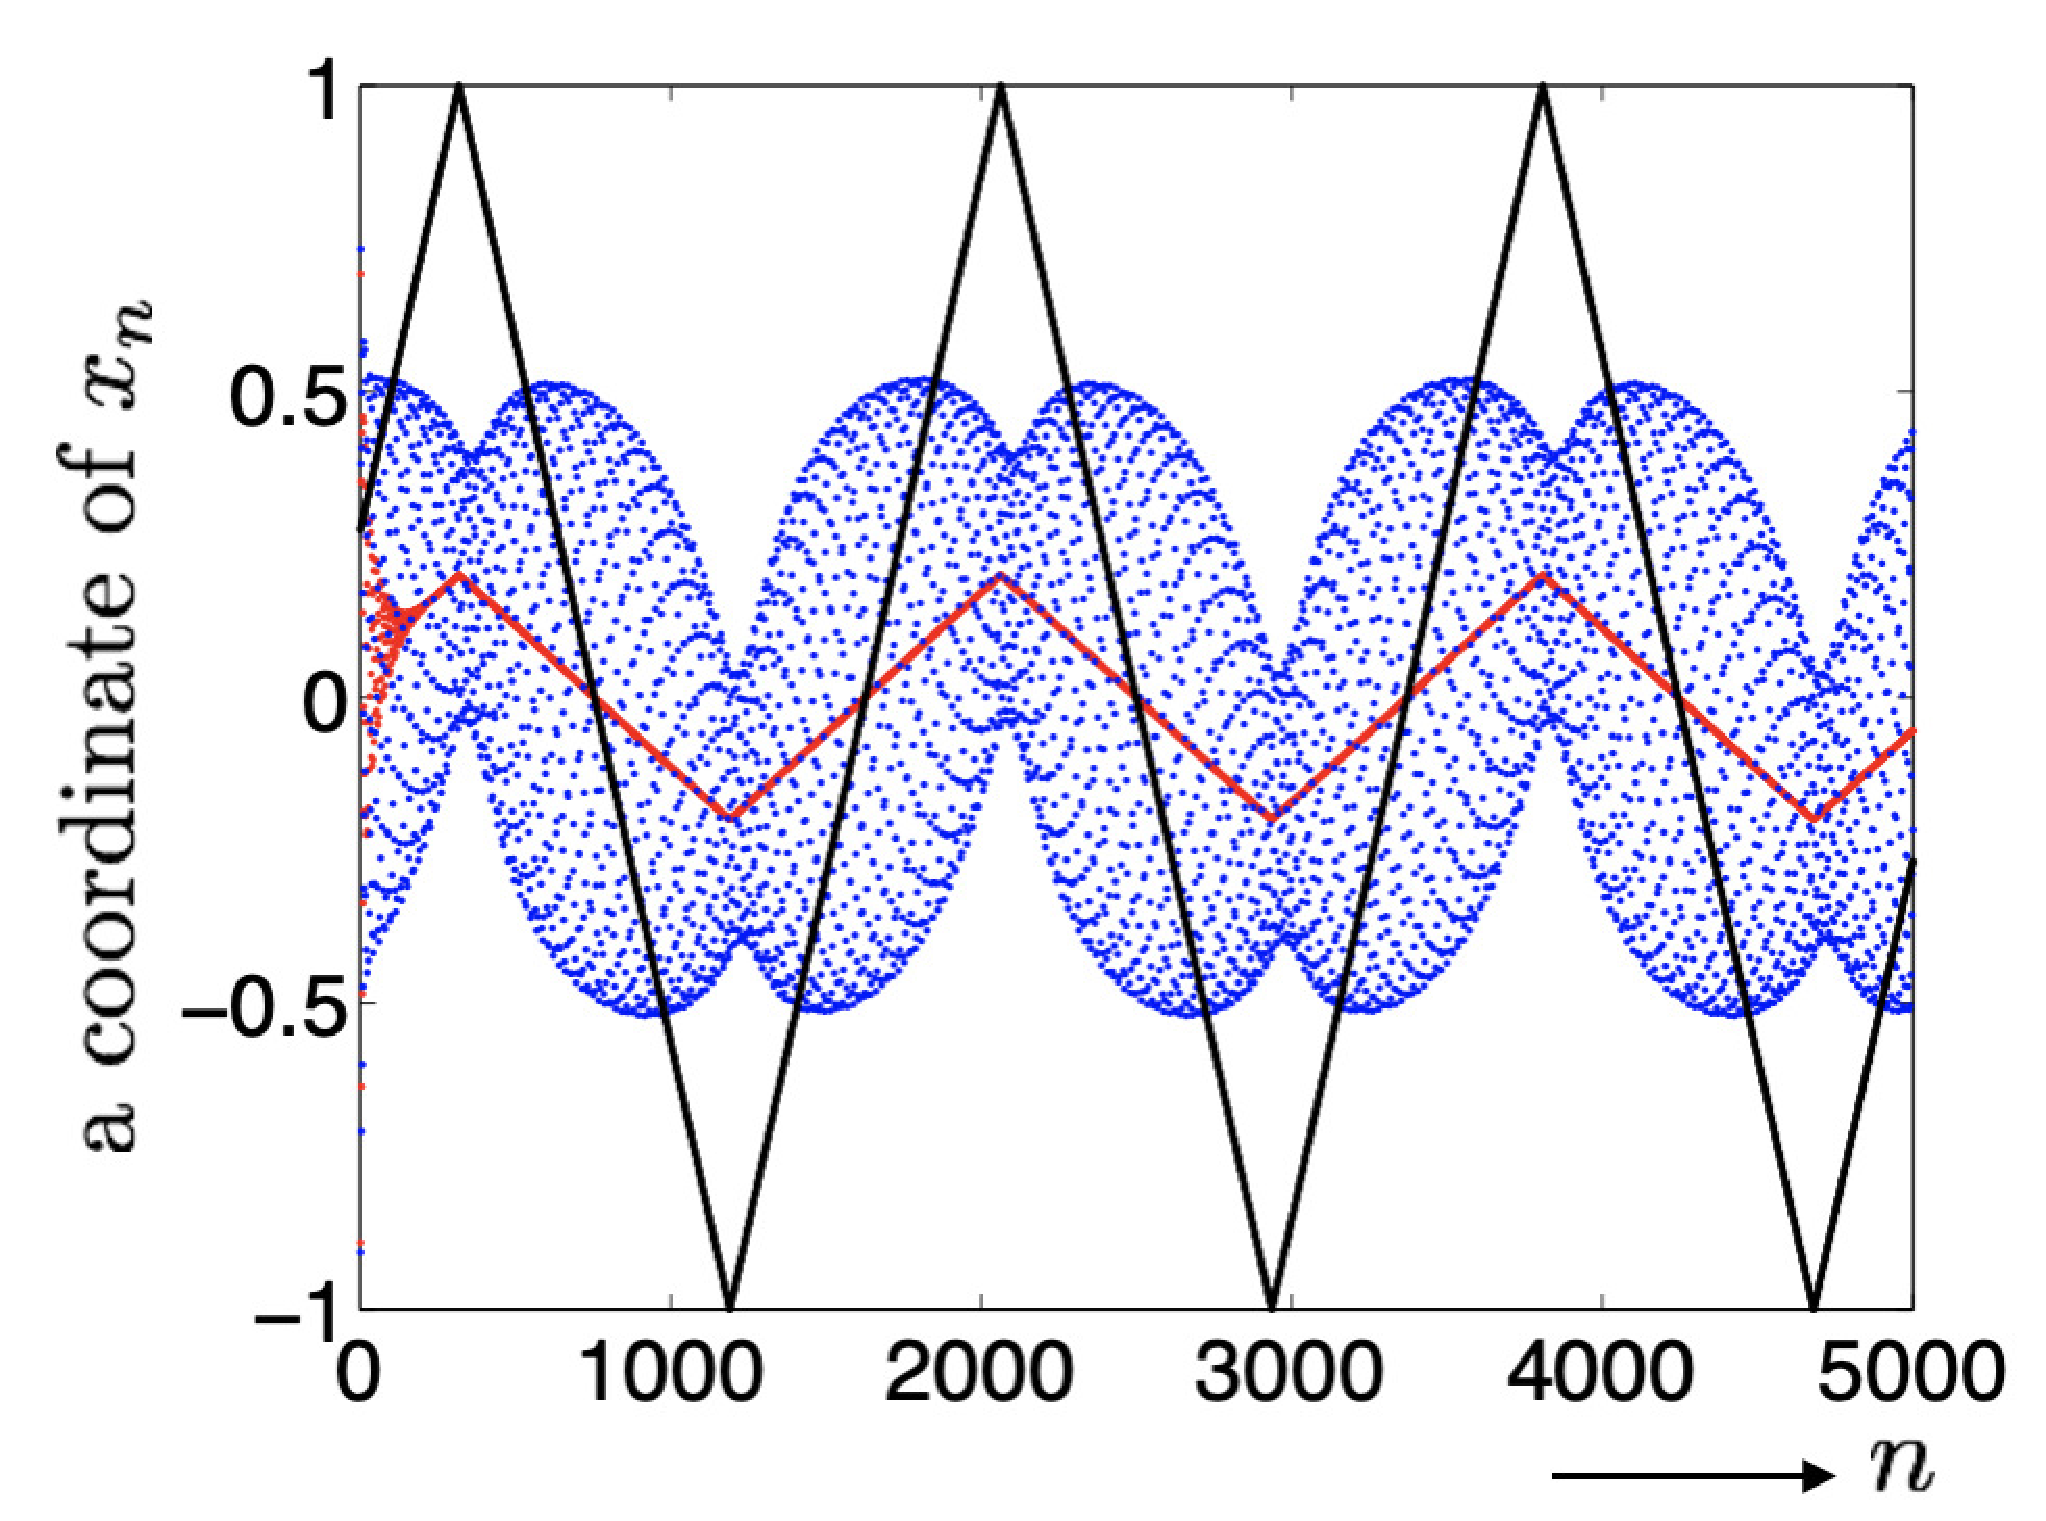
\includegraphics[scale=0.35]{Graphs/_Nonlinearity_Fig_response.eps}
  \centering
\captionof{figure}{A coordinate of a simulated solution $(x_0,x_1,\ldots,x_{5000})$ of a RNN  plotted in red (with parameter $\alpha=0.99$ where $g$ has the USP) and blue ($a=1$, $\alpha=1.05$ where $g$ does not have the USP) while the matrices $A$ and $B$ are randomly generated, and $B$ has unit spectral radius.  Reproduced from~\cite{Manju_Nonlinearity}. } 
\label{fig:memloss_conttime} 
\end{figure} 
\ednote{B: How can I explain the black line? I don't think this makes sense to the reader immediately.}

One may now appreciate an even more astounding result: $g$ having the USP is equivalent to the UAP as is proved in~\cite{Manju_Nonlinearity}.


%We restate the above theorem.

%\begin{Theorem}\label{thm_usp-contr-uap}  The following statements are equivalent:  \vspace{-8mm}  \begin{enumerate}[noitemsep, label=\roman*.]    \item $g$ has the USP.    \item $g$ is a topological contraction.    \item $g$ has the UAP.  \end{enumerate\end{Theorem}{\bf Proof.}  May be found in \cite[Th.1]{Manju_Nonlinearity}

% One need therefore not establish any additional results to ensure that the sequence uniformly approaches the unique solution $\Psi$. This vastly simplifies the effort necessary to set up a problem in order to guarantee that the underlying system will be accurately represented by the conjugate system.

%This also solves the problem of perturbation/noise introduced by the observable or measurement function. Recall from before that an observable is inherently a map that discretises the underlying continuous-time system. Moreover, measurement and device error introduce mistakes. Since we are working with a chaotic system displaying sensitive dependence on initial conditions, these small errors could potentially send the trajectory into a completely different attractor. 
%In the presence of the UAP, however, small measurement errors introduced into the system do not pose the same danger as before since the trajectories will eventually tend towards the actual solution.
% \ednote{(B: Is this Complete enough?)}
% \textbf{From the perspective of perturbation of an autonomous dynamical system, if the resulting nonautonomous system has the USP, then the temporal structure of noise relates to the dynamics on a nonautonomous uniform attractor through a topological semi-conjugacy or a conjugacy.}

\section{The next step in Dynamics}


% Recall that $g$ is only being given inputs from the orbits of $T$.  


%Incredibly, this permits one to initialise a driven system $g$ with an altogether arbitrary initial value $y_m\in{X}$ where $m\in\mathbb{Z}$ and the UAP then guarantees that the sequence $\{y_{m+1}, y_{m+2},\ldots\}$ which satisfies the relation $y_n=g(u_n, y_{n-1})$  for  $k\geq{m}$  will approach the elements $\{x_n\}$ of the actual solution. This vastly simplifies the effort necessary to set up a problem in order to guarantee that the underlying system will be accurately represented by the conjugate system.

We are interested in determining whether $\widehat{T}$ and $G_T$ are related. For this, we introduce  the function $H_2{\overline{}} := (h(r\overline{u}, h(\overline{u})))$ mapping the entirety of a left-infinite sequence to some element in $X\times{X}$. 
Indeed, it may be shown that $g$ having SI-invertibility and the USP immediately guarantees the existence of at least a semi-conjugacy between the systems $(Y_T, G_T)$ and $(\widehat{U}_T, \widehat{T})$.
This is formalised in the Causal Embedding Theorem, which we state next:

\begin{Theorem}
  [\bf Causal Embedding Theorem (adopted from~\cite{Supp})]
  % {\bf (Causal Embedding Theorem.)}
\label{Thm_CET}
	Let $g$ be a driven system with SI-invertibility and the USP. Let $h$ denote the universal semi-conjugacy and $H_2(\overleftarrow{u}) := (h(r\overleftarrow{u}),h(\overleftarrow{u}))$, where $r$ is the right-shift map. 
 Let $(\widehat{U}_T, \widehat{T})$  be the inverse-limit system of a dynamical system $(U,T)$. 
 Then the restriction of $H_2$ to $\widehat{U}_T$ is a topological semi-conjugacy between the inverse-limit system $(\widehat{U}_T, \widehat{T})$ 
and the induced dynamical system  $(Y_T,G_T)$, i.e., the following diagram commutes
\begin{equation} \label{comm_H_CET}
\psset{arrows=->, arrowinset=0.25, linewidth=0.6pt, nodesep=3pt, labelsep=2pt, rowsep=0.7cm, colsep = 1.1cm, shortput =tablr}
 \everypsbox{\scriptstyle}
 \begin{psmatrix}
 \widehat{U}_T & \widehat{U}_T\\%
 Y_T &  Y_T.
 %%%
%  \ncline{1,1}{1,2}^{\widehat{T}} \ncline{1,1}{2,1} <{H_2}
%  \ncline{1,2}{2,2} > {H_2}
%  \ncline{2,1}{2,2}^{G_T}
 \end{psmatrix}
 \end{equation}
or in other words, $(Y_T, G_T)$ is a factor of  $(\widehat{U}_T, \widehat{T})$. Further, if $T:U \to U$ is a homeomorphism, 
then $H_2$ embeds $\widehat{U}_T$ in $X_U \times X_U$, and hence $(Y_T, G_T)$ is conjugate to $(\widehat{U}_T, \widehat{T})$.
\end{Theorem}
{\bf Proof.}  May be found as the proof of~\cite[Th.4]{Supp}

Recall that $H_2$ maps an entire left-infinite solution sequence from $\Psi$ to an element in $X\times{X}$. 
We are drawing nearer and nearer to our principal target and our results carry more and more weight: If we are able to learn $G_T$, we will also have learnt $\widehat{T}$; and since $\widehat{T}$ is an extension of $T$, we will have obtained $T$ as well.  %\ednote{B: Grammarly check}

%\begin{Theorem} Graph \ref{Scomm_h} is exactly the inverse-limit system $(\hat{U}, \hat{T})$.    \end{Theorem}

%We now have the following (which may be compared with \ref{SCausal_H} above):

%\begin{equation} \label{fig:inverse_limsystem}
  %  \[       \psset{arrows=->, arrowinset=0.25, linewidth=0.6pt, nodesep=3pt, labelsep=2pt, rowsep=0.7cm, colsep = 1.1cm, shortput =tablr}      \everypsbox{\scriptstyle}
%      \begin{psmatrix}      \widehat{U}_T  && \widehat{U}_T \\     Y_T && Y_T \\
      %%%
     %  \ncline{1,1}{1,2}^{\widehat{T}} \ncline{1,1}{2,1} <{h}
     %  \ncline{1,2}{2,2} > {H_2}
     %  \ncline{2,1}{2,2}^{G_T}
%      \end{psmatrix}
    %  \]
%  \end{equation}
 

%\begin{Theorem}
 %   $(Y_T, G_T)$ is semi-conjugate to $(\widehat{U}, \widehat{T})$.
%\end{Theorem}
% {\bf Proof.} See \cite[Th.3, Th.4]{manunath2021universal}


\section*{Summarising the discussing thus far:}

It is easy to lose the birds-eye view, so we take a moment to review our progress up until this point.

\vspace{-8mm}
\begin{enumerate}
\item We are interested in a some dynamical system $(U,T)$ with unknown dynamics.
\item To determine properties about this system $(U,T)$ and predict its future evolution, we determine the dynamics of the inverse-limit system $(\widehat{U}, \widehat{T})$.
% Given certain assumptions, we can guarantee that $(\widehat{U}, \widehat{T})$ is at least semi-conjugate to $(U,T)$.
\item If the driven system $g$ is SI-invertible (and $\{u_n\}\in{U}$  is an orbit of $T$), the map $G_T$ exists that describes the single delay dynamics. 
\item If, furthermore, $g$ has the USP, $(Y_T, G_T)$ is semi-conjugate to $(\widehat{U}, \widehat{T})$.
\item If we can assume that $T$ is a homeomorphism, $(Y_T, G_T)$ is topologically conjugate to $(\widehat{U}, \widehat{T})$, an extension space of $(U,T)$
\end{enumerate} 

One can therefore in practice learn the SDD of the driven system states via $G_T$ with enough data thanks to the USP/UAP. This enables us to do at least two things: 
\vspace{-8mm}
\begin{itemize}
\item Forecast  $x_{n+1},x_{n+2}, \ldots$ via iterates of $G_T$ (if $G_T$ can be learnt).
\item Forecast future values of $u_n$ since $x_n$ and $x_{n+1}$ determine $u_n$ since $g$ is SI-invertible. 
\end{itemize} 


Finally, we note that although $G_T$ exists with SI-invertibility, we need the USP as well (see~\ref{fig:pictorialSummary} below for a visual illustration). 
If not, the driven states would have to be running for all time since they would not have forgotten their past states. 

\begin{figure}[ht]
  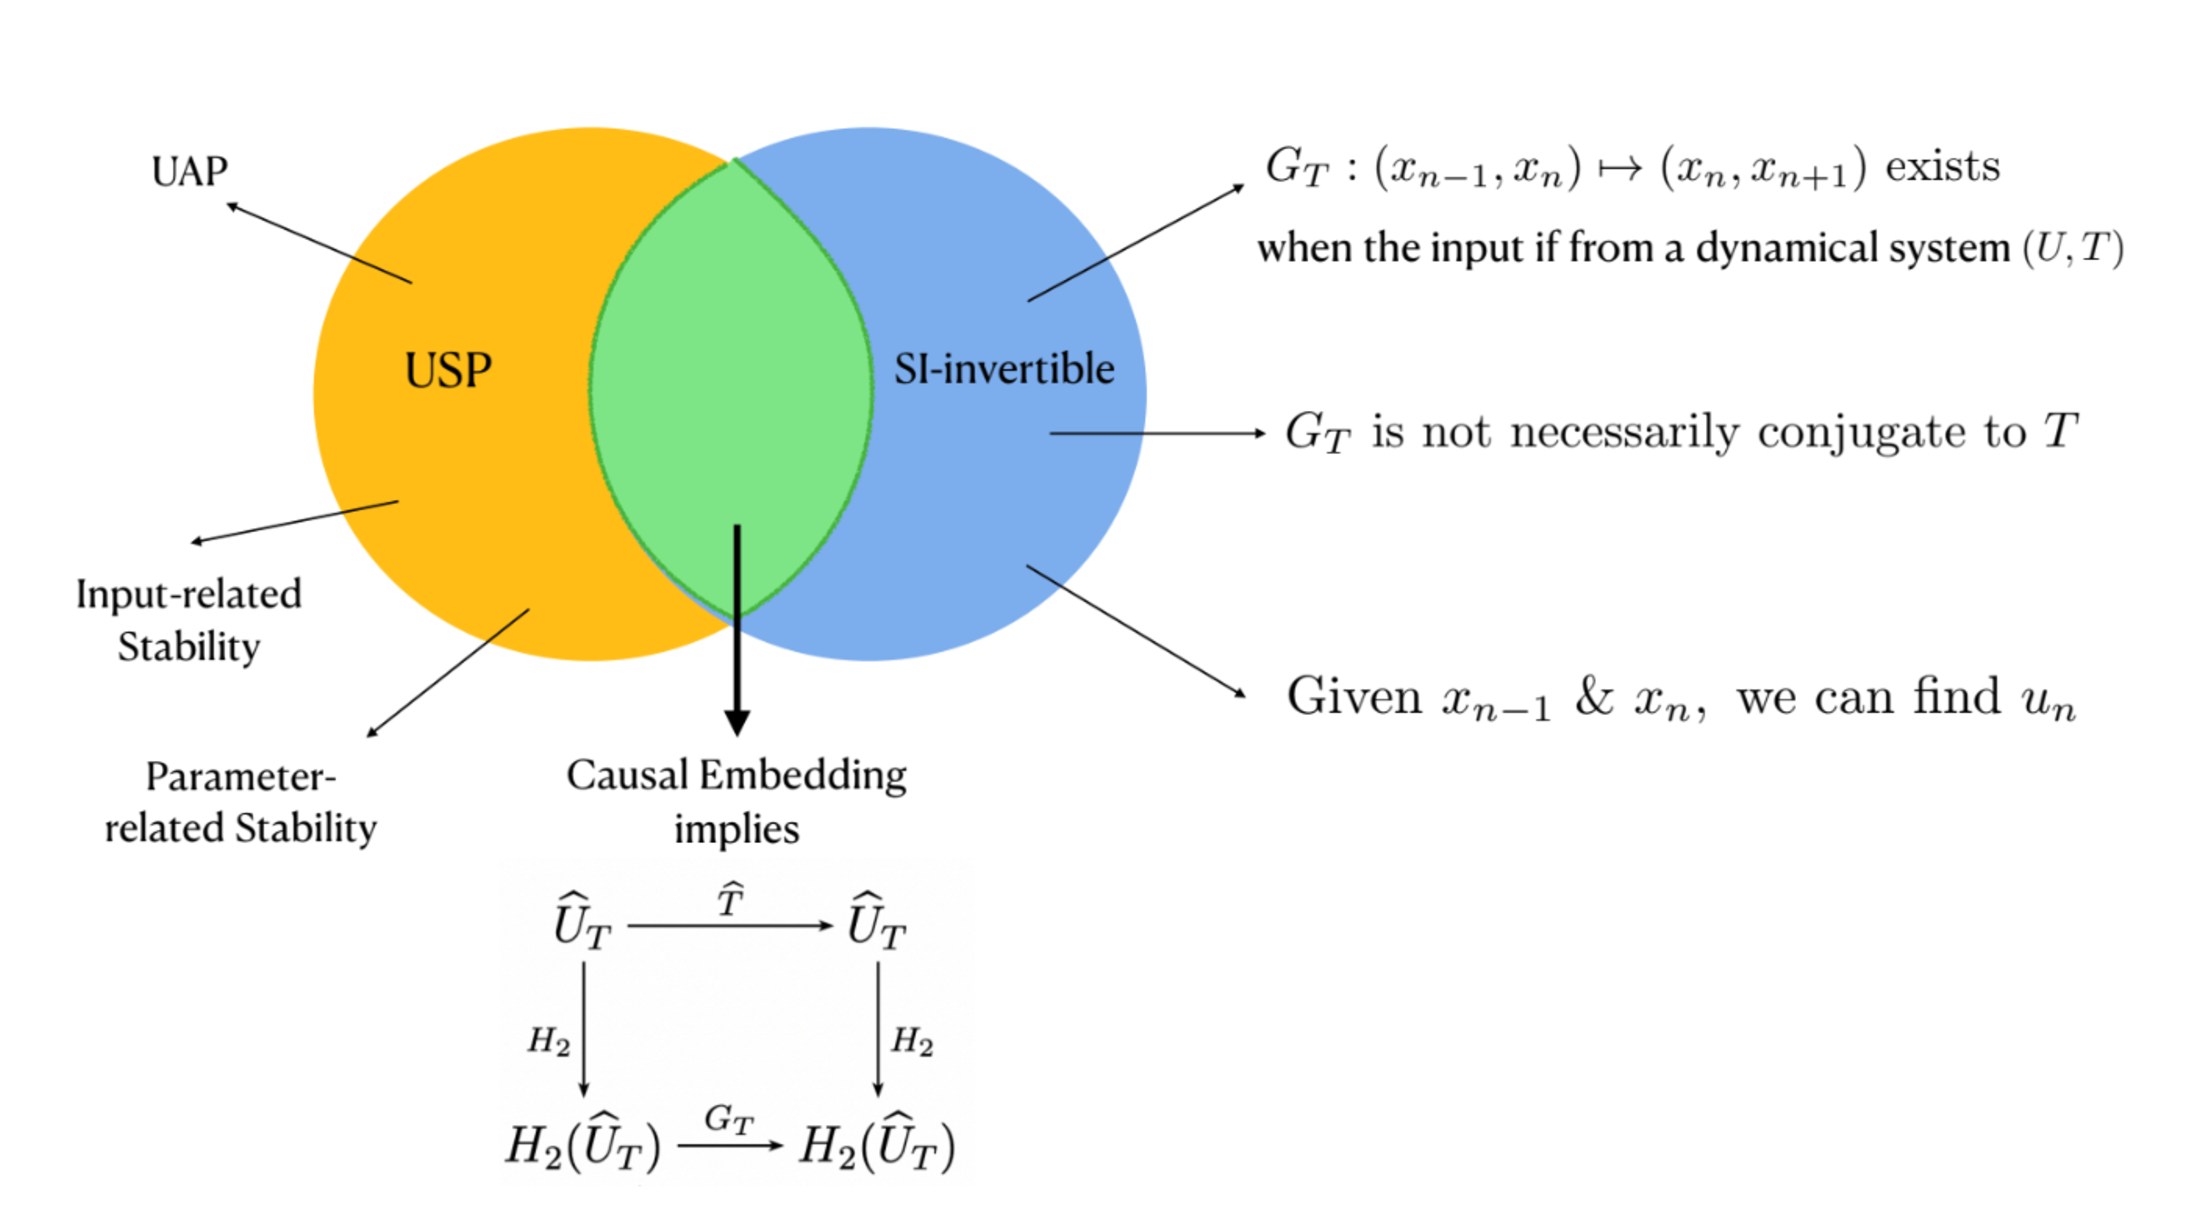
\includegraphics[scale=0.3]{Graphs/_summarypictorial.eps}
  \centering
  \captionof{figure}{Pictorial summary of results obtained up to now and how they overlap. Reproduced from \textbf{(Cite SIG-25May)} }
  \label{fig:pictorialSummary}
\end{figure}
\ednote{Ask M: Cite SIG-25May.}

\section{A discussion of $G_T$ }

In the above sections, we established the map $G_T$ describing the SDD of a driven system. By establishing the existence of this map, we’ve essentially embedded the attractor $U$ (recall from~\ref{attractor_U}) into the higher dimensional space $X\times{X}$.
In layman’s terms, this ensures that there is more “dimensional room” for the underlying system’s underlying dynamics to “move”. Since the dynamics aren’t as “squashed”, we might therefore hope that the dynamics of $G_T$ are in some sense simpler than that of $T$. (Taken note of the fact that $G_T$ is a homeomorphism even when $T$ is just continuous)
 
In~\cite{manjunath2021universal} it is illustrated in an empirical fashion in that the map $G_T$ describes dynamics which are less functionally complex than that of $T$ or of the map $\Phi_{2d,\theta}$. This is done by implementing a Recurrent Neural Network (RNN), which is discussed in Chapter~\ref{ch5}. \ednote{B: Should I add in that we'll be using Pearson coefficient?}
 
We opt to learn $G_T$ in an indirect manner by defining a new map $\Gamma:(x_{n-1},x_n)\mapsto{u_n}$. It will follow immediately from $G_T$’s existence that $\Gamma$ also exists. 

The reasons for taking this roundabout approach remain to be discussed in~\ref{subs_LearnGamma}, but a pat answer may immediately be given: When $\Gamma$ has been learnt, the system can be driven autonomously and then $G_T$ is known anyway. We formalise this with a theorem.

\begin{Theorem}
  When $x_n$ and $x_{n-1}$ are successive points on a solution obtained for input-orbit of $T$ $\{u_n\}$, then the map $\Gamma: X\times{X}\to{U}$ defined by $(x_{n-1},x_n)\mapsto{u_n}$ exists whenever $G_T$ exists 
\end{Theorem}
{\bf Proof.}  See~\cite[Th. 3c]{manjunath2021universal}.

Projection mappings $\pi_i$ are defined in the traditional meaning where a $k$-dimensional vector is projected to it's $i^{th}$ component such that \[\pi_i:(a_1,a_2, \ldotp, a_{k-1}, a_k)\to{a_i}\]

The graph in equation \ref{fig:comm_H_CET} is then extended to the diagram~\ref{Scomm_imp} below:

\begin{equation}  \label{Scomm_imp}
  %    \[ 
      \psset{arrows=->, arrowinset=0.25, linewidth=0.6pt, nodesep=3pt, labelsep=2pt, rowsep=1.3cm, colsep = 1.1cm, shortput =tablr}
   \everypsbox{\scriptstyle}
   \begin{psmatrix}
   \widehat{U}_T & \widehat{U}_T\\%
   Y_T & Y_T\\
   & \textcolor{red}{U \times X}
   %%%
  %  \ncline{1,1}{1,2}^{\widehat{T}} \ncline{1,1}{2,1} <{H_2}
  %  \ncline{1,2}{2,2} > {H_2}
  %  \ncline{2,1}{2,2}^{G_T}
  %  \psset{linecolor=red}
  %  \textcolor{red}{\ncline{2,1}{3,2}<{(\Gamma,\pi_2)}}
  %  \ncline{3,2}{2,2}>{\textcolor{red}{(\pi_2,g)}}.
   \end{psmatrix}
  % \]
  \end{equation} 



The problem finally simplifies to the issue of learning the map $\Gamma$ and combining this with the projection mapping $\pi_2$ and the function $g$, which will be known. A final set of equations is obtained - equations that have been entirely constructed from data.
\begin{eqnarray}\label{eqns_from_data}
	u_{k+1} &=& \pi_1 \circ (\Gamma, \pi_2) \circ (\pi_2,g) (u_k,x_k) \label{Seqn_u}\\
	x_{k+1} &=& \pi_2 \circ (\Gamma, \pi_2) \circ (\pi_2,g) (u_k,x_k). \label{Seqn_x}
\end{eqnarray}



\section{Advantages of learning $\Gamma$}\label{subs_LearnGamma}

One may immediately ask why we opt to take such a roundabout route; why not just learn the map $G_T$ from the get-go? On the surface, this seems to be an arbitrary decision path with no real reasoning, so we take a pause again and discuss the motivation for learning Gamma.
There are a number of distinct advantages. 

In the first place, learning $\Gamma$ saves computational resources. This is due to the fact that the input $u_n$ lies in a lower-dimensional subspace in comparison to the high-dimensional space $X\times{X}$. 

%In practice, if the input is of a  lower dimension, one may easily embed it into the space $X\times{X}$ by padding the vector $u_n$ with zeroes.

Secondly, the function $\Gamma$ is known to be stable. Learning $\Gamma$ makes use of equations~\ref{eqns_from_data} which in turn employs the driven system $g$ possessing the USP, and offers distinct advantages with regards to stability in the presence of perturbation. It is desirable that inputs that differ only slightly would have only ‘slight’ effects on the output of the system. Moreover, one would hope to prevent numerical errors originating from input and measurement noise (see~\cite[Th. 5]{manjunath2021universal}). 
As the data fed into the system is a function of both the input given and the parameters of the system itself (i.e. the value a, $\alpha$ in $\tanh$), we exploit both input-related and parameter-related stability. Both these notions are defined by way of the continuity of an encoding map of an input and design parameter respectively in~\cite{manjunath2020stability}.

Informally, we may consider input-related stability as concerned with the question of whether or not small variations in input would result in small responses.   
If two inputs $\bar{u}$ and $\bar{u}_{noisy}$ are close in the product topology, then their tails could differ greatly due to the metric that generates the product topology has insensitivity to the differences in sequence's tails.
 However if the system has the USP then the function $h$ is continuous and so $h(\bar{u}), h(\bar{u}_{noisy})$ remain close-by for small levels of noise maintaining a measure of robustness to input and measurement noise.\cite{manjunath2021universal}.
In a similar fashion, parameter-related stability is obtained thanks to a result~\cite[Lemma 3.2]{manjunath2020stability} relating this form of stability with the ESP (which is here equivalent to the USP).


% Secondly,  due to $g$ possessing the USP, both input- and parameter-related stability~\cite{manjunath2020stability} is obtained, which in turn prevents numerical errors that caused by input and measurement noise (see~\cite[Th. 5]{manjunath2021universal}). 

Thirdly, learning a chaotic map on a set (here $Y_T$) with even a small measure of noise  means that the learnt system accepts arguments out of the set (Problems similar to Takens, cf.~\ref{sect_takenslimits}). 
We thus have a map $G_T^+$ acting on $Y_T^+$ and since $Y_T$ is not guaranteed to be an attractor of $G_T$ this could lead to errors.
If one learns $G_T$ directly, we are in danger of replicating the problems arising for Takens.  To see this, consider Fig.~\ref{fig:YtGtFailure}.

\begin{figure}[ht]
  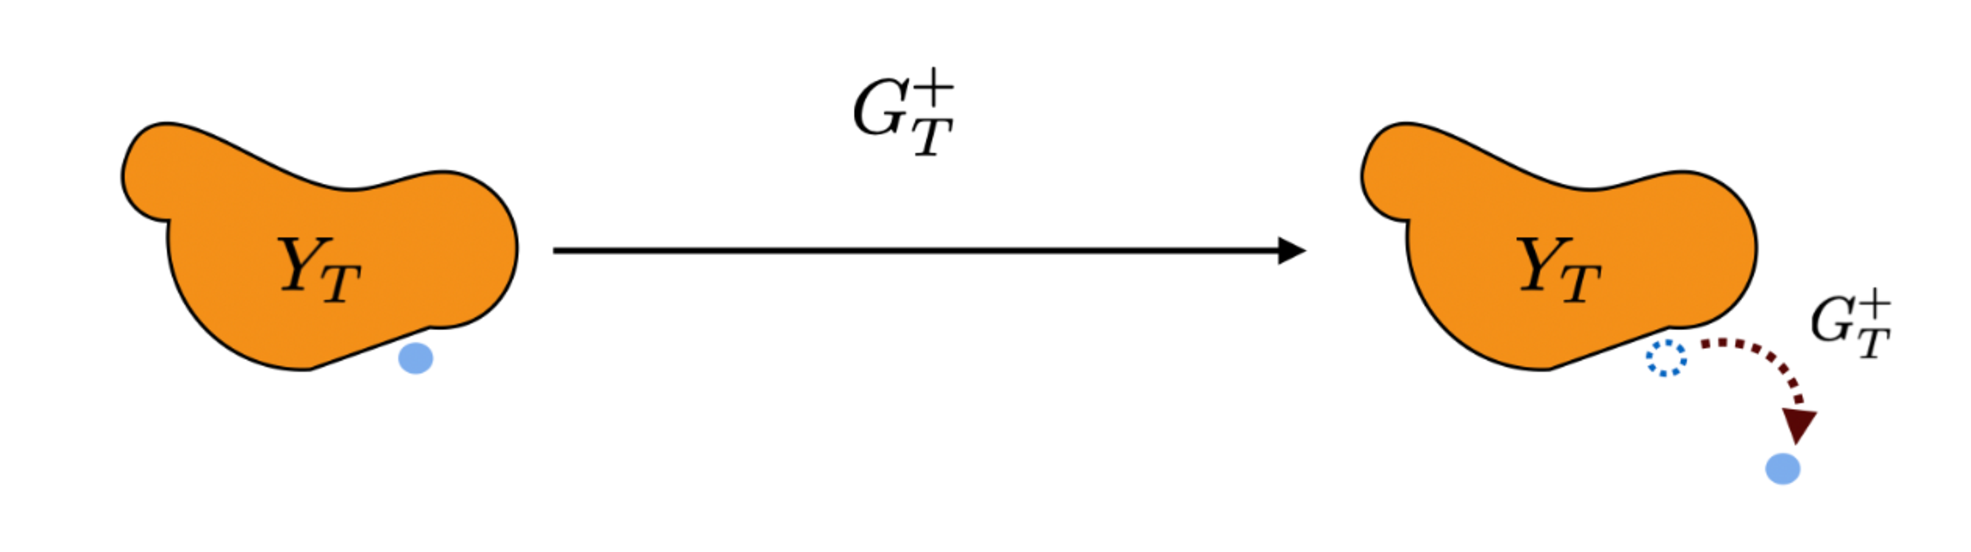
\includegraphics[scale=0.25]{Graphs/_YTerrors.eps}
  \centering
  \captionof{figure}{Diagram of potential errors developing when $G_T$ is learnt.}
\label{fig:YtGtFailure}
\end{figure}

To circumvent this: if a driven system with a saturation function\ednote{B: What is a saturation function?} is used, we can ensure the existence of an attractor $A$ of the map which implements $G_T$, and containing $Y_T^+$ indirectly (via $g$).  \ednote{B: A little vague. Are we saying that an attractor of a map implementing $G_T$ is also the one that contains $Y_T^+$?}
By defining the dynamics to $A$, this prevents large errors from occuring.  
More details on the global dissipativity of $g$, as it is termed there, may be found in~\cite{Supp}.

\begin{figure}[ht]
  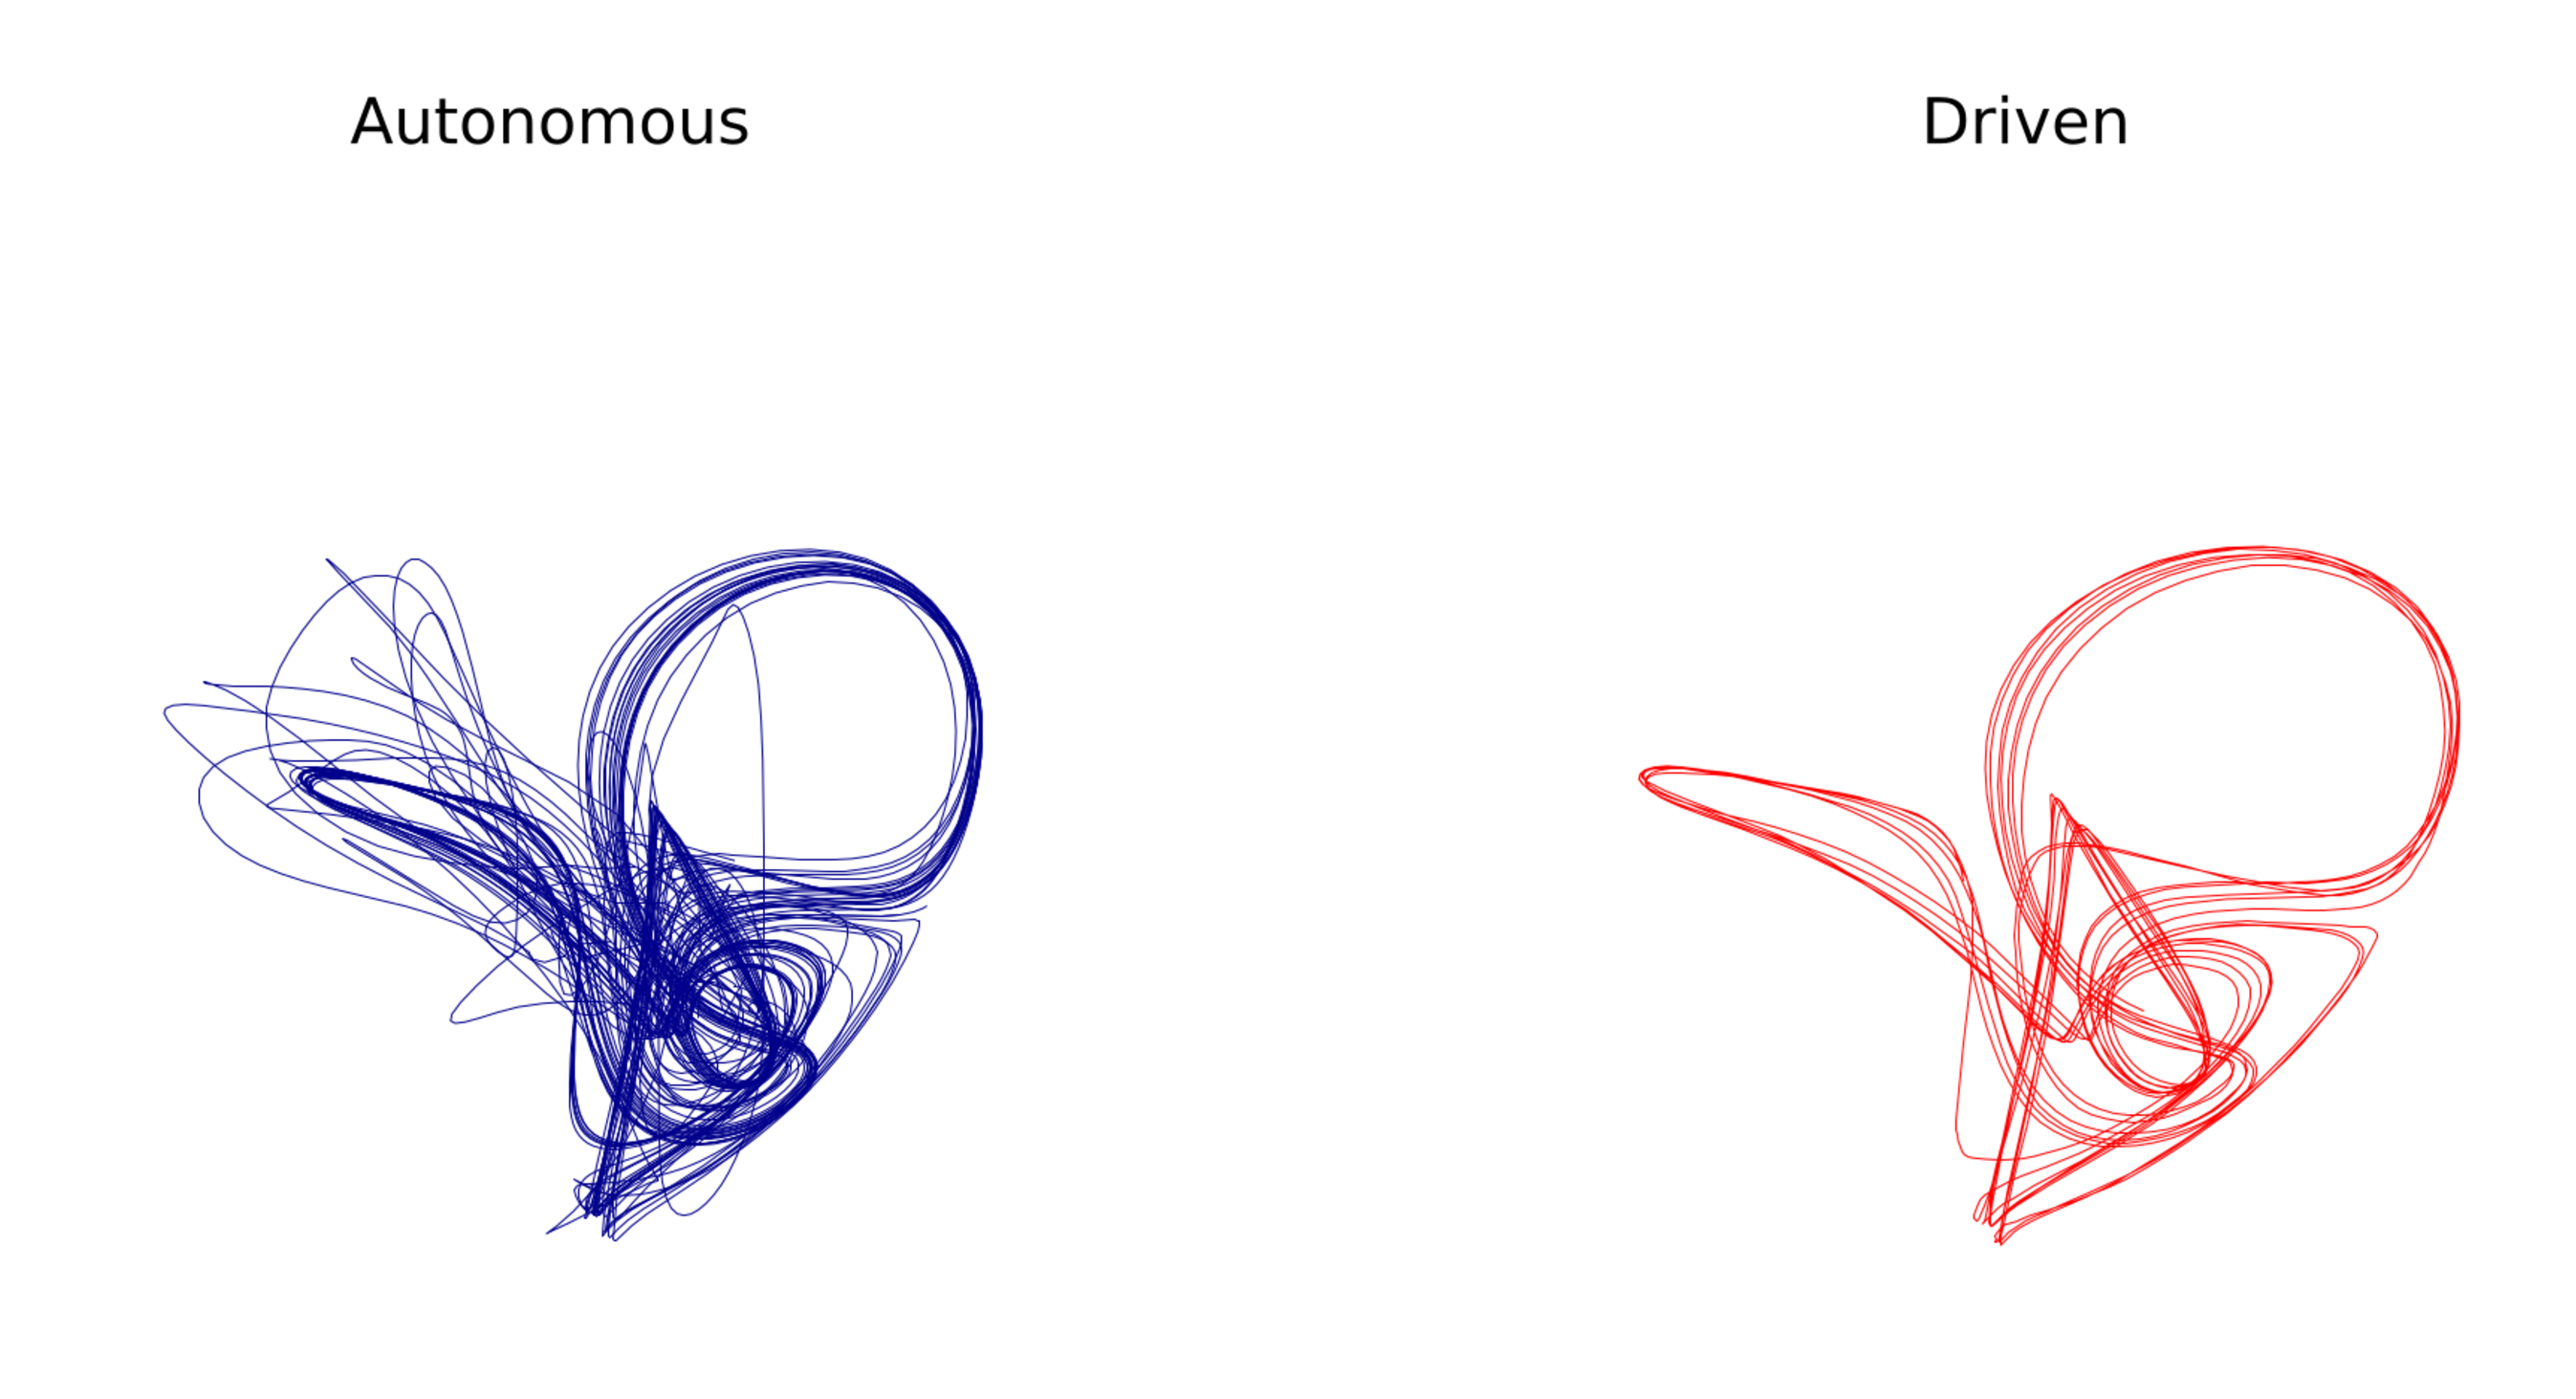
\includegraphics[scale=0.25]{Graphs/_autovsdriven.eps}
  \centering
  \captionof{figure}{Illustrating empirically the importance of global dissipativity. Plotted below are the three principal components of randomly initiated points (blue) of a learnt version of $G_T$ versus the trajectory $(x_{n-1}, x_n)$ (red) of driven states obtained from the Fractal Dream Attractor's data~\ref{Thomas_Attractor}. }
 \label{fig:learningFailure}
\end{figure}

In effect, global dissipativity prevents large numerical errors due to the noise in input data from arising (see Fig.~\ref{fig:learningFailure}). 
If a system is not globally dissipative, neglibly small errors could lead to major inaccuracy which thus induce predictions to utterly fail.

%%%%%%%%%%%%%%%%%%%%%%%%%%%%%%%%%%%%%%%%%%%%%%%%%%%%%%%%%%%%%%%%

